% TODO: add in the referee tag for the submission
%\documentclass[global,twocolumn,referee]{svjour}
\documentclass[global,twocolumn]{svjour}
\usepackage{cite}
\usepackage{amsmath}
% \usepackage{amsthm}
\usepackage{amsfonts}
\usepackage{url}
\usepackage{comment}
\usepackage{paralist}
\usepackage{graphicx}
\graphicspath{{./figs/}} 
\usepackage{listings}
\usepackage[usenames,dvipsnames,svgnames,table]{xcolor}
\usepackage{flushend}
\usepackage{hyperref}
\usepackage[firstpage]{draftwatermark}

\definecolor{dkgreen}{rgb}{0,0.6,0}
\definecolor{mauve}{rgb}{0.58,0,0.82}
\definecolor{light-gray}{gray}{0.88}

\lstdefinestyle{myML}
{frame=none,
  basicstyle=\ttfamily,
  language=ML,
  aboveskip=3mm,
  belowskip=3mm,
  showstringspaces=false,
  columns=flexible,
  numbers=none,
  numberstyle=\tiny\color{gray},
  commentstyle=\color{dkgreen},
  stringstyle=\color{mauve},
  breaklines=false,
  breakatwhitespace=true,
  tabsize=2,
  linewidth=2\linewidth
}

\lstdefinestyle{agree}
{frame=none,
  basicstyle=\ttfamily,
  language=ML,
  aboveskip=3mm,
  belowskip=3mm,
  showstringspaces=false,
  columns=flexible,
  numbers=none,
  numberstyle=\tiny\color{gray},
  commentstyle=\color{dkgreen},
  stringstyle=\color{mauve},
  breaklines=false,
  breakatwhitespace=true,
  tabsize=2,
  linewidth=2\linewidth,
  morekeywords={eq, bool, guarantee, assume, true, false, pre, not, and, or, property, const}
}

\hyphenation{op-tical net-works semi-conduc-tor}

\newcommand{\konst}[1]{\ensuremath{\mathsf{#1}}}
\newcommand{\imp}{\Rightarrow}
\newcommand{\lval}{\ensuremath{\mathit{lval}}}
\newcommand{\set}[1]{\ensuremath{\{ {#1} \}}}
\newcommand{\kstar}[1]{\ensuremath{{#1}^{*}}}
\newcommand{\Lang}[1]{\ensuremath{{\mathcal L}({#1})}}
\newcommand{\LangTheta}[1]{\ensuremath{{\mathcal L}_{\theta}({#1})}}
\newcommand{\itelse}[3]{\mbox{$\mathtt{if}\ {#1}\ \mathtt{then}\ {#2}\ \mathtt{else}\ {#3}$}}

\newcommand{\figref}[1]{Fig.~\ref{#1}}

% Latex trickery for infix div operator, from stackexchange

\makeatletter
\newcommand*{\bdiv}{%
  \nonscript\mskip-\medmuskip\mkern5mu%
  \mathbin{\operator@font div}\penalty900\mkern5mu%
  \nonscript\mskip-\medmuskip
}
\makeatother

\newcommand{\ie}{\textit{i.e.}}
\newcommand{\eg}{\textit{e.g.}}
\newcommand{\etal}{\textit{et al.}}
\newcommand{\etc}{\textit{etc.}}
\newcommand{\adhoc}{\textit{ad hoc}}

% \theoremstyle{plain}
% \newtheorem{theorem}{Theorem}
% \newtheorem{lemma}{Lemma}

% \theoremstyle{definition}
% \newtheorem{definition}{Definition}

% \theoremstyle{remark}
% \newtheorem{remark}{Remark}

\journalname{Software and Systems Modeling}

\begin{document}
\title{
  Synthesizing Verified Components for Cyber Assured Systems Engineering
  \thanks{DISTRIBUTION STATEMENT A.  Approved for public release.}
}

\author{
  Eric Mercer\inst{1}    \and 
  Konrad Slind\inst{2}   \and
  Isaac Amundson\inst{2} \and
  Darren Cofer\inst{2}   \and
  Junaid Babar\inst{3}   \and
  David Hardin\inst{3}
}

\institute{
  Brigham Young University        \\
  Provo, Utah                     \and
  Applied Research and Technology \\ 
  Collins Aerospace               \\
  Minneapolis, Minnesota          \and
  Applied Research and Technology \\ 
  Collins Aerospace               \\
  Cedar Rapids, Iowa
}

\date{Received: date / Revised version: date}

\maketitle

\begin{abstract}
Cyber-physical systems, such as avionics, must be tolerant to
cyber-attacks in the same way they are tolerant to random faults: they
must gracefully recover, or safely shut down, as requirements dictate.
We have developed a workflow for creating, and inserting,
high-assurance components implementing cyber-resiliency into a
model-based systems engineering environment.  Example high-assurance
components are filters, which guard against malformed input, and
runtime monitors, which guard against spoofing and other malicious
behavior. A formal specification in the form of a \emph{code contract}
defines each high-assurance component and is developed with the
support of \emph{test contracts} for testing the specified behavior.
Once tested, model checking used to verify that the added
high-assurance component indeed addresses system-level cyber
requirements.  Implementations for these high-assurance components are
directly synthesized from their code contracts and are backed up by
proofs showing that high-level specifications map in a
semantics-preserving way to code generated by a verified compiler.  We
report on a case study that cyber-hardened a UAV system by inserting
high assurance components to harden the open source Air Force Research
Laboratory's OpenUxAS services for route planning.  The case study
demonstrates that synthesizing correct implementations from code
contracts is feasible in real-world systems engineering.

\end{abstract}

\section{Introduction} \label{sec:intro}

\egm{Add to introduction and related work, that what is done at
Galois called Copilot. Its a stream processing langague that generates
code from the specification. Copilot to C. Effectively CodeGen from
Lustre. Bounds how far needed to look in past for any value.}

In recent years, aerospace stakeholders have realized that avionics
systems are subject to possible cyber-attacks just like other
cyber-physical systems.
%
\footnote{This work was funded in part by the
Defense Advanced Research Projects Agency (DARPA).  The views
expressed are those of the authors and do not reflect the official
policy or position of DARPA or the U.S. Government.}
%
Thus, in addition to being fault-tolerant, safety-critical avionics
systems must also be {\em cyber-resilient}.  Cyber-resiliency means
that the system is tolerant to cyber-attacks just as safety-critical
systems are tolerant to random faults: they recover and continue to
execute their mission function, or safely shut down, as requirements
dictate.

Unfortunately, systems engineers are currently given few development
tools to help answer even basic questions about potential
vulnerabilities and ways to mitigate vulnerabilities.  They instead
rely on process-oriented checklists and guidelines.  Cyber
vulnerabilities are often discovered during penetration testing late
in the development process; or worse yet, they may be discovered only
after the product has been fielded, necessitating extremely expensive
and time-consuming remediation. This is not a sustainable development
model.

%% The DARPA Cyber Assured Systems Engineering (CASE) project is targeted
%% at developing tools for design, analysis, and verification that enable
%% systems engineers to {\em design-in} cyber-resiliency for complex
%% cyber-physical systems.

We have been developing the {\em BriefCASE} toolsuite to address this need.
\brfcs\ is a Model-Based Systems Engineering (MBSE) environment
built in the Open Source AADL\footnote{AADL is the acronym for
Architecture Analysis and Design Language~\cite{aadl}.}  Tool
Environment (OSATE) to add new design, analysis, and code generation
capabilities for building cyber-resilient systems.

In this paper we describe how \brfcs\ facilitates inserting,
specifying, testing, and synthesizing high assurance components into a
system to improve its cyber-resiliency.  The main organizing concept
is that of an architecture-to-architecture \emph{security-improving
transform}, achieved via the insertion of a new architectural
component aimed at mitigating a cyber-vulnerability.  We describe two
cyber-resiliency transformations in this paper: (1) the insertion of a
filter to prevent malformed data from a malicious actor being
propagated to downstream components, and (2) the insertion of a
runtime monitor to detect (and alert) unexpected behaviors arising
from untrusted components.

A code contract is a formal specification in the Assume Guarantee
Reasoning Environment (\agr) language.
\agr\ is a compositional reasoning verification engine that uses \emph{contracts} on components to specify input and output properties and then prove whether or not those properties hold when given a sub-component implementation \cite{agree2013}.
The code contract language is Turing complete allowing the designer to
specify arbitrarily complex behavior.  These contracts are unit tested
for correctness with \emph{test contracts}.  Test contracts define
test scenarios to be implemented by the code contract under test.
\agr\ proves whether or not that code contract implementation is correct, enabling the designer to iteratively test the component behavior inside the \brfcs\ environment.
Once the behavior of the code contract is verified, \agr\ proves that---due to the newly
included high-assurance components---the hardened system meets its
cyber-resiliency requirements.

Another novel aspect of our workthe approach discussed in this manuscript is
the synthesis of the code contracts for the high-assurance components
to \ckml, a verified compiler implementation for the functional
programming language ML \cite{cakeml}.  This manuscript describes in
detail the synthesis path from code contracts to \ckml\ code,
providing a formal framework in which to argue correctness. \ckml\
then provides a verified compilation path to several different target
binaries (and also proving that the meaning of the \ckml\ source code
is exactly preserved in the final binaries).  A key contribution here
is that the code contract semantics are defined in such a way that
the \agr\ verification results for the code contract hold for the
deployed component, \ie, the component will detect and prevent the
indicated cyber-vulnerabilities over all possible finite
inputs. Preliminary work has shown how to lift this result to infinite
input traces as these systems are inherently reactive and intended to
run forever~\cite{case-verified-filter}, \cite{cakeml-space-cost}.

The manuscript further details a case study applying these
transformations with \brfcs\ to an Unmanned Aerial Vehicle (UAV)
system that uses the Air Force Research Laboratory's OpenUxAS services
for route planning.  OpenUxAS, as an open source product, is
considered \emph{untrusted}.  The UAV system is thus transformed to be
resilient to malicious behavior that may arise in the untrusted
component.  Here the transforms add filters to guard against malformed
input and monitors to guard against malicious flight plans from
OpenUxAS. The case study system is complex and shows the viability of
the approach in potential full-scale industrial design.

\brfcs\ is open source and publicly available \cite{fmide} as are the examples and case study discussed in this manuscript \cite{repo, phase2, camkes, case}.
Our approach currently applies to common cyber-vulnerabilities, such
as overflow, lack of input validation, and supply-chain issues;
however, other cyber-vulnerabilities such as side-channel attacks and
denial of service are not yet dealt with in our work.  Here, we do not
report on the invention of a new type of high-assurance component in
terms of capability; instead, our contribution is in the automated
synthesis of security-improving components from formal specifications
and a means to show that the synthesis is correct.

We now give a summary of the contributions detailed in this
manuscript.
\begin{compactitem}
  \item The language and semantics of code contracts to specify the behavior of high assurance components.
  \item Test contracts as a stylized mechanism to unit test code contracts inside the \brfcs\ framework with \agr.
  \item A synthesis path from code contracts to \ckml\ with a formal framework to argue correctness.
  \item A formal argument that \agr\ verification of code contracts carry over to the resulting binaries from the \ckml\ compiler.
  \item A case study that used the implementation of the approach in \brfcs\ to add cyber-resiliency to a non-trivial UAV system.
\end{compactitem}
The rest of this manuscript is organized as follows.
\secref{sec:overview} is an overview of the \brfcs\ environment and key tools in that environment relative to the contributions of this work. The approach is illustrated by a simple example in
\secref{sec:example}. Essential background on \agr\ verification and specification are
presented in \secref{sec:agree}.
The language and semantics of code contracts are defined in \secref{sec:code-contracts}, and test contracts are defined in \secref{sec:testing}.
The synthesis pathway is covered in Section~\ref{sec:synthesis}.
\secref{sec:case-study} discusses the case study.
This is followed by related work in \secref{sec:related-work}.
The conclusions and future work are in \secref{sec:conclusion}.

\begin{comment}
  BriefCASE incorporates model-level cyber analysis tools (presently
  GearCASE~\cite{gearcase2020} and DCRYPPS~\cite{dcrypps2019}) which can
  examine AADL models for potential vulnerabilities and suggest
  cyber-security requirements to mitigate them.  A library of
  architectural transforms guides the system engineer through automated
  model transformations that modify the architecture to address these
  requirements, possibly inserting new high-assurance components into
  the system.  Implementations for the new components are synthesized
  from formal specifications using
  SPLAT~\cite{slind-hcss2020},~\cite{formal-filter-synth-langsec}
  (Semantic Properties for Language and Automata Theory).


  Formal
  verification that the transformed system model meets its requirements
  is accomplished via \agr~\cite{agree2013} (Assume Guarantee Reasoning
  Environment).
  %The AGREE analysis \emph{assumes} properties on the inputs of a given component of the system, and attempts to formally prove the conjectured \emph{guarantees} of the output.
  \agr\ is a {\em compositional assume-guarantee} style model checker
  for AADL models that attempts to prove properties about one layer of
  an architecture using properties allocated to its subcomponents.
  Cyber-resilient code implementing the verified model is then
  automatically generated using the High Assurance Modeling and Rapid
  Engineering for Embedded Systems (HAMR) toolkit~\cite{hamr}.  If
  desired, this code can be targeted to the formally verified seL4
  secure microkernel~\cite{sel4-2009}.
\end{comment}

\subsection{SOSYM Journal Details}
The submission must have 30\% new material over what was published in MODELS 2021.
There is no page limit.
The article will go through a full review cycle.
The due date is \textbf{March} $1^\mathrm{st}$, \textbf{2022}.

\noindent The summary of the discussion regarding how the MODELS publication might be extended is given below.
\begin{compactitem}
  \item Expand the case study with the TA6 models
  \item Expand the case study with an actual full AGREE specification
  \item AGREE formal semantics summary including the uninterpreted functions
  \item Strengthen the assurance argument from AGREE to binary by way of CakeML
  \item Expand related work (add recent work published after 2018). 
  \item Respond more fully to the reviews from MODELS (see below).
\end{compactitem}

\noindent The summary of items from the MODELS reviews.
\begin{compactitem}
  \item Add recent work published after 2018
  \item Add discussion on the limitation of the approach: what attacks can and cannot be covered, can valid messages be rejected, etc.
  \item Expand the role of Briefcase in the case study with input examples to provide more proof of the proposed model's effectiveness on the hardened system (e.g., show a malformed line search task, it's filter, and why it works) 
  \item Clarify research questions answered by the case study and make the figures bigger
  \item Discuss what efforts are optimized with the automations versus a fully manual process for creating the components--how does the automated transformation affect actual time for engineers
  \item Without verifying the correctness of the transformations, can prevention of certain attacks be guaranteed?
\end{compactitem}
\section{Simple Example} \label{sec:example}
Show a filter, monitor, and gate form Phase II and indicate each of their intended roles.

\section{AGREE Contract Specification} \label{sec:agree}
The goal of this section is to illustrate in more detail the process a
system designer follows to add cyber requirements to the AGREE
specifications and then automatically transform the system to insert
the high-assurance components. The AGREE specifications generated by
the transforms for the high-assurance components are
explained. The section ends with a concise formal statement of the
meaning of an AGREE specification for a high-assurance component. This
meaning is what must be preserved by the synthesis.

\newsavebox{\sw}
\begin{lrbox}{\sw}
\begin{lstlisting}[style=agree]
eq req : bool = event(AutomationRequest);
eq avl : bool = event(AirVehicleLocation);
eq wp : bool = event(Waypoint);
eq rsp: bool = event(Start);
eq alrt : bool = event(Alert);

assume "Automation request is well-formed" :
    req => WELL_FORMED_AUTOMATION_REQUEST(AutomationRequest);
assume "Air vehicle location is well-formed" :
    avl => WELL_FORMED_WAYPOINT(AirVehicleLocation);

eq current : bool = (req = rsp);
eq previous : bool = (req and not rsp) ->
                      pre(req and not rsp) and (not req and rsp);
eq policy : bool = current or previous;
eq since : bool =  alrt or (alrt and (false -> pre(since)));

guarantee "Start includes a waypoint" :
    rsp => wp;
guarantee "Locations required after the start waypoint" :
    (wp and not rsp) => avl;
guarantee "Waypoint is well-formed" :
    wp => WELL_FORMED_WAYPOINT(Waypoint);
guarantee "Alert if start is not bounded relative to a request" :
    policy or since;
\end{lstlisting}
\end{lrbox}

\begin{figure}
  \begin{center}
    \scalebox{0.60}{\usebox{\sw}}
  \end{center}
  \caption{The SW component contract.}
  \label{fig:sw}
\end{figure}

The AGREE specification for the SW component in the example of Section~\ref{sec:example} with the added cyber requirements is given in \figref{fig:sw}. The AGREE specification language is a first-order predicate calculus that uses stream concepts, and operators, from the Lustre language \cite{10.1145/41625.41641}. As with Lustre, the semantics are synchronous data-flow where the inputs, outputs, and expressions are characterized by data streams that comply with the input assumptions. The semantics are such that the contracts are evaluated in dependency order with inputs being propagated to outputs through all the contracts until they stabilize; as such, the contracts, and thereby the top-level model, must be acyclic. Once the contracts have stabilized, the model takes a synchronous step to the next input data in the stream. The semantics do not model computation or communication delay. The output of one contract is seen at the input of any downstream contract in the same step of the input data stream.

The AGREE model checker attempts to prove several properties of the top-level model being verified. The first is that the output guarantees of each component implementing the system are strong enough to validate the input assumptions of any downstream component as well as to satisfy the guarantees of the output of the top-level component being verified (i.e., the system composition meets input assumptions at each input as well as the guarantees on the system output). These properties are reported in the expanded lists in \figref{fig:example}(b) and \figref{fig:hardened}(b).  The next set of properties prove that the contract specifications for each component are self-consistent (i.e, a contract does not contradict itself). These are the unexpanded results at the bottom of the figures.

Returning back to the contract in \figref{fig:sw}, it uses \texttt{eq} statements to define variables local to the contract specification. For example, the \texttt{req} variable is equivalent to the \texttt{event(AutomationRequest)} expression. In the AGREE semantics, there is an implicit \emph{event} input (or output) associated with every named event port in a component. The semantics used here do not buffer these events so the implicit input (or output) is only a boolean value. An \texttt{event} expression refers to that implicit input (or output) and is true when data is placed on the named port. The system contract here states assumptions on well-formed input, followed by guarantees on properties about the output.

The \emph{Alert if start is not bounded relative to a request} guarantee is an invariant on the expression \texttt{policy or since}, meaning that either the policy holds or the alert is sounding. The \texttt{policy} is defined by two local values: \texttt{current} and \texttt{previous}. The \texttt{current} value is asserted when in the current time step there is a request with a response, or there is no request and no response.

The value of \texttt{previous} in the current time step relies on values from the previous time step. The \texttt{->} operator designates initialization, as the previous time step is undefined in the first step of the system. The left operand to the operator is the initial value of \texttt{previous} at start, which in this example is \texttt{(req and not rsp)}, because seeing a request with no response is inconclusive in the first step of the system. The right operand is the value of \texttt{previous} after the initial step. Here the \texttt{pre} operator refers to the value of the expression \texttt{(req and not rsp)} in the prior time step, \texttt{previous} is true if the previous time step made a request without a matching response and the current time step has the matching response to that request with no new request.

The value of \texttt{since} in \emph{Alert if start is not bounded relative to a request} relies on its own value in the previous time step. The intuitive reading of the expression is that the alert has been true since the time when it first sounded. The first \texttt{alrt} sets \texttt{since} to true, and once the value of \texttt{since} is true, that value persists as long as \texttt{alrt} holds. The \emph{Alert if start is not bounded relative to a request} guarantee defines one requirement of a cyber-hardened system implementation. Together with the other guarantees, the contract models the expected input and output of the system as a whole.

\begin{figure}
  \begin{center}
    \begin{tabular}{c}
      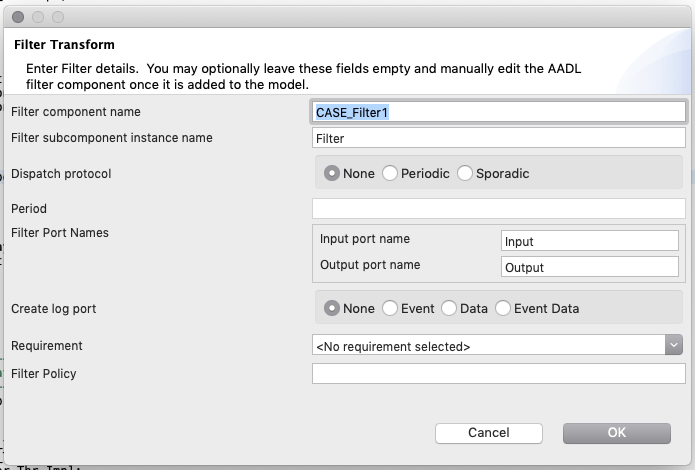
\includegraphics[scale=0.3]{dialogue.png}
    \end{tabular}
  \end{center}
  \caption{Wizard for automatically transforming the model with a filter.}
  \label{fig:dialogue}
\end{figure}

\newsavebox{\flt}
\begin{lrbox}{\flt}
\begin{lstlisting}[style=agree]
eq policy : bool =
  WELL_FORMED_AUTOMATION_RESPONSE(Input);
guarantee Filter_Output "Filter output is well-formed" :
  if event(Input) and policy then
    event(Output) and Output = Input
  else not event(Output);
\end{lstlisting}
\end{lrbox}

\newsavebox{\mntr}
\begin{lrbox}{\mntr}
\begin{lstlisting}[style=agree]
const is_latched : bool =
  Get_Property(this, CASE_Properties::Monitor_Latched);
eq rsp : bool = event(Response);
eq req : bool = event(Request);
eq current : bool = (req = rsp);
eq previous : bool = (req and not rsp) ->
                      pre(req and not rsp) and (not req and rsp);
eq policy : bool = current or previous;
eq alert : bool = (not policy)
                -> ((is_latched and pre(alert)) or not policy);
guarantee Monitor_Alert
  "Alert port tracks alert variable" :
  event(Alert) = alert;
guarantee Monitor_Output
  "Output if not alerted" :
  if event(Alert) then (not event(Output)) else
  if event(Response) then (event(Output) and (Output = Response))
  else (not event(Output));
\end{lstlisting}
\end{lrbox}

\begin{figure}
  \begin{center}
    \begin{tabular}{c}
      \scalebox{0.60}{\usebox{\flt}} \\
      (a) \\
      \scalebox{0.60}{\usebox{\mntr}} \\
      (b)
    \end{tabular}
  \end{center}
  \caption{High-assurance component contracts. (a) The filter. (b) The monitor.}
  \label{fig:assurance}
\end{figure}

As noted previously, the original system fails to guarantee the cyber requirements. BriefCASE provides two transformations to address the failing requirements: inserting a filter and inserting a monitor. The component is added by selecting the connection in the model where the high-assurance component is to be added, and then choosing the appropriate transformation. The system designer can provide transform configuration parameters in a wizard, as shown in \figref{fig:dialogue}. The policy of the high-assurance component can be stated directly in the wizard, or it can be left  blank. In this example, the policy is specified as \texttt{WELL\_FORMED\_AUTOMATION\_RESPONSE(Input)}.
Additionally, because a transformation is ultimately driven by a cyber requirement, BriefCASE updates an embedded Resolute assurance case~\cite{resolute-destion}.  Resolute keeps track of the evidential artifacts necessary for supporting the requirement, and can be run at any time to determine whether those artifacts are valid.
%Additionally, the filter can be attached to any requirement the vulnerability analysis. This association is useful the the assurance case from the Resolute tool [CITE DESTION 2021]. The \emph{OK} button creates the component and inserts it accordingly into the implementation

The AGREE contract specification generated by the transform is shown in \figref{fig:assurance}(a). The guarantee is stylized for synthesis and completely defines the meaning of the output under every possible input.
%A similar dialogue exist for inserting monitors that allows the system designer to add and remove inputs as needed.
The resulting AGREE specification for the monitor in this example is shown in \figref{fig:assurance}(b). The \texttt{is\_latched} value makes the alert persistent, meaning that once the alert is raised, it is always raised.  This behavior is one of the several options available in the dialogue. The definition for \texttt{policy} is taken by the system developer from the contract in \figref{fig:sw}. As before, the guarantees for the outputs are autogenerated by the tool and completely define each output under every possible input.

\subsection{Brief Semantics Definition}

Here the formal semantics of the AGREE contract specification are briefly
presented to make clear the meaning of a high-assurance component. 
These semantics are used in the next section to argue that the synthesis
preserves the same input to output behavior as the AGREE specification.

Assume that all data is in its raw form which is a contiguous sequence of bytes
representing exactly what is sent over a wire by the communication fabric, so a
datum is given by a \konst{string}. This assumption is important to the 
correctness argument in the next section. An \emph{environment},
$\theta: \lval \mapsto \konst{string}$, binds \emph{L-values} to strings where 
an L-value is anything that can appear on the left-hand side of an assignment
such as a named port, a field in a record, a entry in an array, a local
value defined by an eq-statement etc. 

Let $s$ be an AGREE contract specification for some high-assurance
component. The notation $\theta_s$ is used to denote the environment that
contains a binding for any L-value in the scope of $s$ and nothing else, and
the notation $\Theta_s$ denotes the universe of all such environments. The
semantics of $s$ are defined over streams, $\pi = \theta_1, \theta_2, \ldots$, which
are finite sequences of environments, $\pi \in \Theta_s^*$. 

\begin{comment}
[\emph{So basically $\theta$ covers the inputs and the state, i.e. we can
generate a contig type for the inputs plus state vars.} ]

[Question: what is a \emph{total} environment? One that supplies at
least the bindings in $\theta$ needed to evaluate the spec?]
\end{comment}

The function $\konst{eval}\; s\; \pi$ is defined such that it evaluates $s$ on
the stream, $\pi$, and returns \konst{true} if $s$ is invariant along the
entire stream and \konst{false} otherwise. A guarantee in $s$ is invariant if
its associated expression is true in the context of every step of the stream, while
an eq-statement in $s$ is invariant if its binding in the context of every step
is equivalent to the computed value of its associated expression in that same
context. All guarantees and eq-statements must be invariant in the stream for
the function to return \konst{true}.

The meaning of an AGREE contract
specification is now defined as the set of environment streams on which it is invariant.
%
\[
  \mathcal{L}(s) = \set{\pi \in \Theta_s^* \mid \konst{eval}\ s\ \pi = \konst{true}}
\]
%
\noindent Intuitively, any stream $\pi \in \mathcal{L}(s)$, at each step, binds
the L-values in the eq-statements
in a way that is consistent with their associated expressions and the guarantees are all
true in that same step.

We claim that a synthesized high-assurance component preserves the input to output
relationship in the specification $s$ over every stream in $\mathcal{L}(s)$. 
Let $\pi^\prime
= \konst{SynthEval}\ s\ \pi$ denate a function that synthesizes $s$ and then
evaluates that synthesized component on the stream $\pi$ to create a new
stream $\pi^\prime$ containing added output and other bindings. We
say that two streams, $\pi_a = \pi_b$ are equivalent in regards to a
specification $s$ if and only if the two streams are the same length and
agree on bindings for the input and output for $s$ at every step of the streams.
We now formally state the correctness claim for synthesis.
%
\[
  \forall \pi \in \mathcal{L}(s)\ ((\konst{SynthEval}\ s\ I_s(\pi)) =_s \pi)\\
\]
%
where $I_s(\pi)$ returns the corresponding stream that only retains bindings
for inputs in each step and nothing else. The claim is that the synthesized component
generates the same output stream as the specification for any stream
belonging to the specification that is restricted to just input binding at each step.

\section{Synthesis} \label{sec:synthesis}
Synthesis maps from model and specifications to code. The synthesis
algorithm traverses the system architecture looking for occurrences of
filter and monitor specifications;  for each such occurrence it
generates a CakeML program. In the following, we examine both filter
and monitor synthesis. The latter is typically much more involved, and
we will therefore devote more attention to it.

\subsection{Filter Generation}

A filter is intended to be very simple; it is expected to have one
input port and one output; messages on the input that the filter
policy admits pass unchanged to the output port; all others are
dropped (not passed on). We have explored in our work two kinds of
filter. In the first, a relatively shallow scan of the input buffer
can enforce the policy. For example, we have used the expressive power
of Contiguity Types \cite{contiguity-types} to enforce
\emph{lightweight} bounds constraints on GPS coordinates in UxAS
messages. On the other hand, the second kind of filter will parse the
input buffer into a data structure specified in AGREE and apply an
user-defined \emph{well-formedness} property, also specified in AGREE,
to the data. This allows arbitrarily complex well-formedness checking.

The decision of a filter is made and performed within one thread
invocation. Thus, in its given time slice, the filter does the following:

\begin{enumerate}

\item checks to see if there is any input available; if there is none
then it yields control; otherwise,

\item the input is read (and parsed if need be),

\item the wellformedness predicate is evaluated,

\item if the predicate returns \konst{true} then the input buffer
 is copied to the output; otherwise no action is taken, and

\item the filter yields control
\end{enumerate}

\begin{remark}[Partiality]

The role of partiality should be emphasized: steps 2 and 3 can fail;
the data might not be parseable or the wellformedness computation
could be badly written and fail at run time. In such cases, the filter
should recover and yield control without passing the input onwards. In
these cases, the filter is behaving as it should, but there are also
cases in which a correctly specified filter would not meet its
specification at runtime. This situation arises when the
filter \emph{ought} to accept a message, but lack of resources result
in the filter failing to do so. Examples of this would be, for
example, if the parse of a message needed more space than allocated;
another example would be if the timeslice provided by the scheduler is
too small for the wellformedness computation to finish.

\end{remark}


{\emph{Need some discussion of filters and their step-wise properties
  in relation to their infinitary properties. Reference to Johannes'
  work.}

\newsavebox{\contig}
\begin{lrbox}{\contig}
\begin{lstlisting}[style=myML]
  Waypoint =
    {Latitude  : f64
     Longitude : f64
     Altitude  : f32
     Check     : Assert
      (~90.0 <= Latitude and Latitude <= 90.0 and
       ~180.0 <= Longitude and Longitude <= 180.0 and
       1000.0 <= Altitude and Altitude <= 15000.0)}

  AutomationResponse =
    {TaskID : i64
     Length : u8
     Waypoints : Waypoint [3]}
\end{lstlisting}
\end{lrbox}

\begin{figure}
  \begin{center}
    \begin{tabular}{c}
      \scalebox{0.60}{\usebox{\contig}}
    \end{tabular}
  \end{center}
  \caption{Contiguity type specification for filter.}
  \label{fig:filter-contig}
\end{figure}


\newsavebox{\cml}
\begin{lrbox}{\cml}
\begin{lstlisting}[style=myML]
fun filter_step () =
 let val () = Utils.clear_buf buffer
     val () = API.callFFI "get_input" "" buffer
 in
    if WELL_FORMED_AUTOMATION_RESPONSE buffer
    then
      API.callFFI "put_output" buffer Utils.emptybuf
    else print"Filter rejects message.\n"
end
\end{lstlisting}
\end{lrbox}

\begin{figure}
  \begin{center}
    \begin{tabular}{c}
      \scalebox{0.60}{\usebox{\cml}}
    \end{tabular}
  \end{center}
  \caption{Synthesized CakeML for the filter.}
  \label{fig:filter-cakeml}
\end{figure}

The contiguity type specification for the filter is shown in
\figref{fig:filter-contig}. The synthesized CakeML code for the filter is shown in
\figref{fig:filter-cakeml}. The code is called at dispatch by the
scheduler. The \texttt{API.callFFI} is the link to the communication
fabric to capture input and provide output. The body of the function
restates the filter contract to make the appropriate assignments in a
way that matches the truth value of the predicate in the filter
guarantee.  The auto-generated AGREE specification raises an alert
output when the relation is violated.

% A \emph{system} is a collection of \emph{components}, \emph{connections}
% between components, a \emph{scheduler} to order execution, and a
% \emph{system environment} for primary inputs.

\subsection{Monitor Generation}

Monitors, since they are intended to track and analyze the externally
visible behavior of system components through time, require more
computational features than filters. In particular, our conception of
a monitor is a predicate on its input (and output) streams, being able
to access the value of a stream at any earlier point in time, if
necessary. Thus monitors commonly use state to keep track of earlier
values, unlike filters which are stateless. This reasoning leads us to
specify the computation for a monitor component by a step function of
the following form:
\[
\konst{stepFn} : \mathit{input} \times \mathit{stateVars} \to \mathit{stateVars} \times \mathit{output}
\]
Thus, in its given timeslice, a monitor evaluates the \konst{stepFn} on its inputs and the current values of the state variables. In detail, it takes the following steps:

\begin{enumerate}

\item each available input is parsed into data of the type specified
by the port type;

\item the stateful variables in $\mathit{stateVars}$  are evaluated in dependency order.

\item values of outputs are computed

\item outputs are written and the new state is written

\item control is yielded
\end{enumerate}

Our earlier remarks on partiality apply here too, of course.


The scheduler \emph{activates} components in some order.It is an
obligation on the system that the scheduler follows some sensible
partial order of component activation and allows each component
sufficient time for its computation.  Activating a monitor component
takes the form of the following pseudo-code:
\[
\begin{array}{ll}
 \mathit{(i_1,\ldots)} & = \konst{readInputs}(); \\
 (v_1,\ldots) & = \konst{readState}() ; \\
 ({v_1}',\ldots), ({o_1}',\ldots) & = \konst{stepFn} ((i_1,\ldots),(v_1,\ldots)) ; \\
 \multicolumn{2}{l}{\konst{writeState}({v_1}',\ldots);} \\
 \multicolumn{2}{l}{\konst{writeOutputs}({o_1}'\ldots);} \\
\end{array}
\]

\paragraph{Initialization}
A monitor may need to accumulate a certain minimum number of
observations before being able to make a meaningful assessment of
behavior. Until that threshold is attained, the monitor is essentially
in a kind of \emph{initialization} phase. In order for correct code to
be generated, monitor specifications need to spell out the values of
output ports when in an initialization phase. For example, suppose a
monitor does some kind of differential assessment of inputs at
adjacent timeslices, alerting when (say) the measured location of a
UAV at times $t$ and $t+1$ is such that the distance between the two
locations is unusually large. Such a monitor needs two measurements
before making its first judgement, but at the time of its first
output, only one measurement will have been made. The specification
for must explicitly state what the correct first output is.


\section{UxAS Case Study} \label{sec:case-study}
In this section, we apply the BriefCASE tool to the development of a UAV surveillance system in which a UAV receives commands from a ground station to conduct surveillance along a geographical feature such as a river. The on-board mission computer then generates a flight plan consisting of a series of waypoints that the UAV must traverse to complete its mission. The UAV is also given a set of \textit{keep-in} and \textit{keep-out} zones that may constrain its flight path.

We have modeled the system architecture of the UAV in AADL.  It includes a Mission Computer for communicating with the ground station and generating flight plans, and a Flight Control Computer for UAV navigation.  The Mission Computer architecture model includes hardware components such as a processor, memory, and communication devices, as well as software.
%
The initial software architecture model (shown in Figure~\ref{fig:sw-initial}) contains drivers for communication with the Ground Station and Flight Control Computer, a Waypoint Manager component that provides flight plan coordinates to the Flight Control Computer, and the Flight Planner.  The Flight Planner is the open-source UxAS software developed by AFRL~\cite{uxas}. 

For this application, UxAS accepts three types of messages.  The \textit{Operating Region} message defines where the UAV can and cannot fly.  The \textit{Line Search Task} message contains a series of waypoints that the UAV should traverse.  The waypoints typically lie along some geographical feature of interest, such as a river or railway.  Note that the UAV may not be able to directly traverse the Line Search Task waypoints due to no-fly zone constraints specified in the Operating Region message.  Anytime after receiving the Operating Region and Line Search Task messages, a ground station can transmit an \textit{Automation Request} message, which instructs UxAS to generate a flight plan that satisfies these constraints.  UxAS passes the flight plan in an \textit{Automation Response} message to the Waypoint Manager.  Because the Flight Control Computer can only process a small number of waypoints at a time, the Waypoint Manager parcels a small number of waypoints corresponding to the current UAV position, and sends them to the Flight Control Computer over a serial connection via the UART Driver.

\begin{figure}[h]
	\centering
	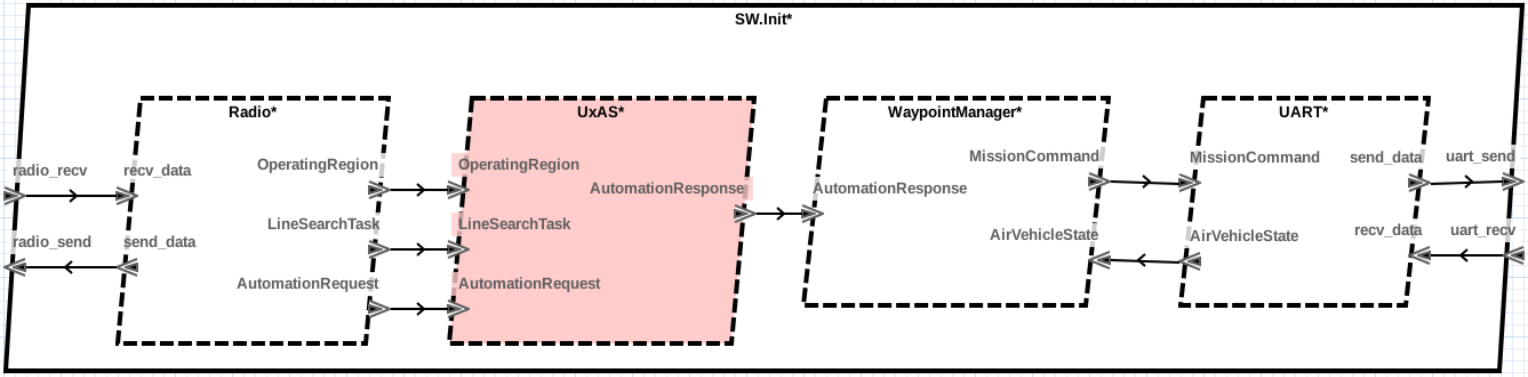
\includegraphics[width=1\columnwidth]{figs/sw-initial.png}
	\caption{Initial software architecture.} 
	\label{fig:sw-initial} 
\end{figure}

Within the software model, we have formalized some of the high-level requirements as assume-guarantee contracts.  We perform a formal analysis using the AGREE tool (which is integrated with the BriefCASE environment) to verify that the model satisfies the contracts.  For the initial version of our design, the verification passes.
%
Although we are satisfied with the results of the formal verification using AGREE, we have not yet analyzed the design for cyber-vulnerabilities.  
In BriefCASE, we analyze the model using one (or more) of the integrated cybersecurity analysis tools.  The tools generate a list of new requirements corresponding to cyber vulnerabilities found in the design.  To satisfy these requirements we need to mitigate the vulnerabilities discovered by the analysis by modifying the design.
%
For example, because we annotated the open-source UxAS component as \texttt{uncontrolled} (colored red in Figure~\ref{fig:sw-initial}), the cyber analysis tools generate requirements for ensuring unverified or malicious code (that could potentially be included in the component) will not impact other processes. 

In total, seven cyber requirements are generated and imported into our model.  These include four \textit{well-formedness} requirements, two requirements for \textit{monitoring} the behavior of the open-source UxAS component, and an \textit{attestation} requirement for ensuring the Ground Station software has not been tampered with.  Requirements are imported into the model as goals in a Resolute assurance case.  Because we can run Resolute at any time during development, we can easily determine for a given snapshot of the model which requirements are not yet supported by evidence.

The intent of the \textit{well-formedness} requirements is to prevent malformed messages from causing a buffer overrun or code injection attack.  In the UAV design, such messages are most likely to originate from a remote source or the uncontrolled UxAS component.  By placing filters on the connections upstream of mission-critical components, such attacks could be mitigated.  The Filter transform is therefore applied for each well-formedness requirement, inserting filter components on the incoming and outgoing UxAS connections.  

The filter behavior for each component is specified in AGREE.  Not only does this enable formal verification within the modeling environment, but it also provides a means for synthesizing the component implementation in a provably correct manner using the SPLAT tool.  Because SPLAT is integrated with BriefCASE, the proof it emits when synthesizing component code is used as evidence in the Resolute goal for the corresponding mitigation.  When Resolute evaluates whether such a goal is supported by evidence, it checks for the existence of the synthesis proof in addition to verifying the architecture is correct.  

The AGREE filter policies for the four UxAS connections are similar, and check that record values contained in the messages are within appropriate ranges.  For example, the Automation Response message filter, which drops message containing malformed flight plans, is defined as shown in Figure~\ref{fig:automation-response-filter}.  Although Latitude, Longitude and Altitude are defined as 64-bit \textit{reals}, the filter ensures only messages containing waypoint values between [-90,9], [-180,180], and [0,15000], respectively. 

\begin{figure}[h]
	\centering
	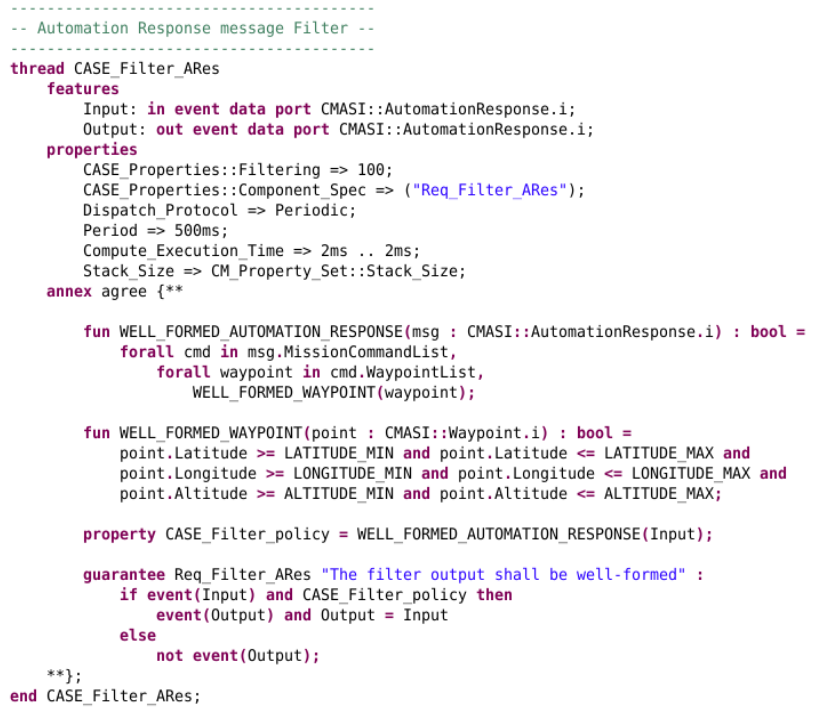
\includegraphics[width=1\columnwidth]{figs/automation-response-filter.png}
	\caption{Automation Response Filter specification.} 
	\label{fig:automation-response-filter} 
\end{figure}

In addition to monitoring the UxAS output for malformed messages, we must also monitor for suspicious behavior.  This requires adding components for detecting that UxAS has crashed, as well as monitoring the correctness of the flight plans it produces.  The Monitor transform is applied for this class of mitigation.  In general, monitors observe a channel and compare its contents against a reference signal or constant.  The monitor policy specifies acceptable comparisons, and if violated, the monitor sends out an alert.  A monitor can choose to \textit{gate} the observed signal, in which case it also acts as a special kind of filter and drops the message if the policy is violated.  The \textit{monitoring} requirements drive two transforms.  The first adds a \textit{response} monitor to send an alert if UxAS does not emit a response within a set amount of time from receiving a request.  The second adds a \textit{geofence} monitor to ensure that generated flight plans are compliant with the specified keep-in and keep-out zones.  The Geofence Monitor is a gated monitor; it prevents the observed Automation Response message from reaching the Waypoint Manager. 

Similar to the filters, the monitor policies are specified in AGREE. For example, 
%The Response Monitor specification is shown in Figure~\ref{fig:response-monitor}, and 
the Geofence Monitor specification is shown in Figure\ref{fig:geofence-monitor}. 

% \begin{figure}[h]
% 	\centering
% 	\includegraphics[width=1\columnwidth]{figs/response-monitor.png}
% 	\caption{Response Monitor specification.} 
% 	\label{fig:response-monitor} 
% \end{figure}

\begin{figure}[h]
	\centering
	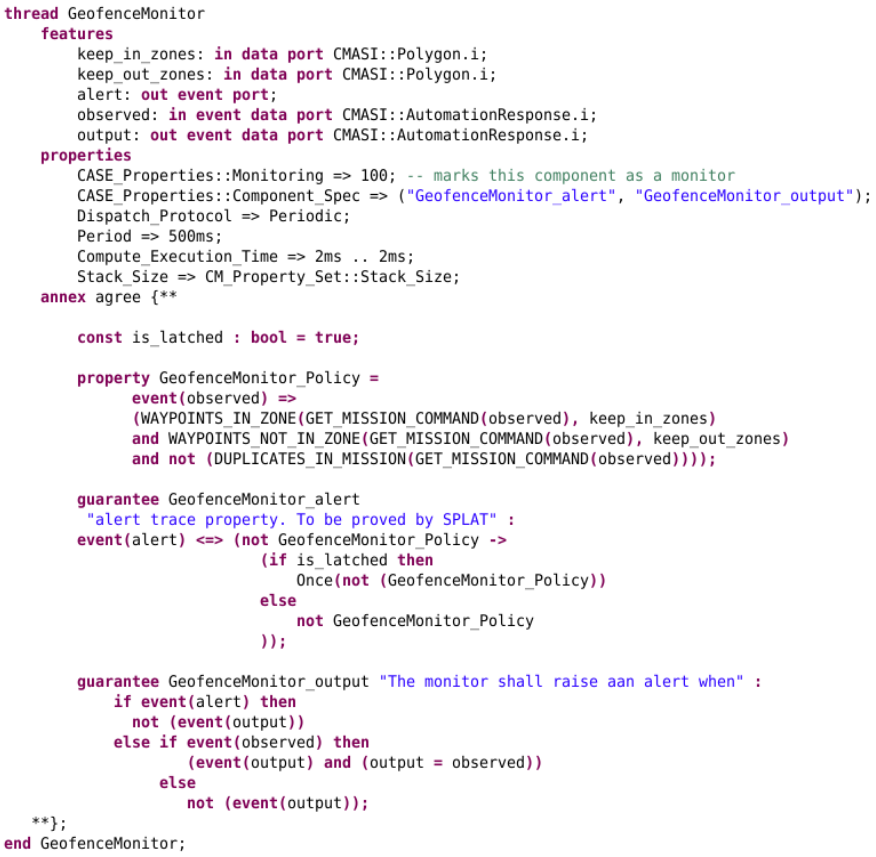
\includegraphics[width=1\columnwidth]{figs/geofence-monitor.png}
	\caption{Geofence Monitor specification.} 
	\label{fig:geofence-monitor} 
\end{figure}

The requirements that have been addressed so far mitigate vulnerabilities related to malformed messages and malicious behavior \textit{on board} the UAV.  But we also want to protect against a compromised Ground Station that could potentially transmit well-formed, but malicious commands. The final cyber-requirement is mitigated by the Attestation transform~\cite{attestation-copland}, which adds two components to the UAV software: an Attestation Manager for evaluating remote systems like the Ground Station, and an Attestation Gate for filtering messages from sources that have not been approved by the Attestation Manager.  The Attestation Manager is implemented in CakeML and automatically inserted into the application code base by BriefCASE.  Because the Attestation Gate acts as a filter, the transform automatically generates its complete AGREE specification.%, as shown in Figure~\ref{fig:attestation}.

% \begin{figure}[h]
% 	\centering
% 	\includegraphics[width=1\columnwidth]{figs/attestation.png}
% 	\caption{Atestation specification.} 
% 	\label{fig:attestation} 
% \end{figure}

After transforming the model to address the cyber requirements, the software architecture now appears as shown in Figure~\ref{fig:hardened-sw}.  The components in green were added to the model by way of an automated BriefCASE transform and are critical for mitigating cyber attacks. 
We formally verify the model with AGREE to show that all of the component contracts are satisfied, including the new contracts introduced during the model transformations.
Because it is imperative that these high-assurance component implementations are correct,
we run the SPLAT tool to produce provably-correct code.  
The synthesized code is output to a directory in the build file system with the location specified for each component in the model.  The corresponding correctness proof is used in our assurance case as additional evidence that the vulnerability has been properly mitigated.

\begin{figure}[h]
	\centering
	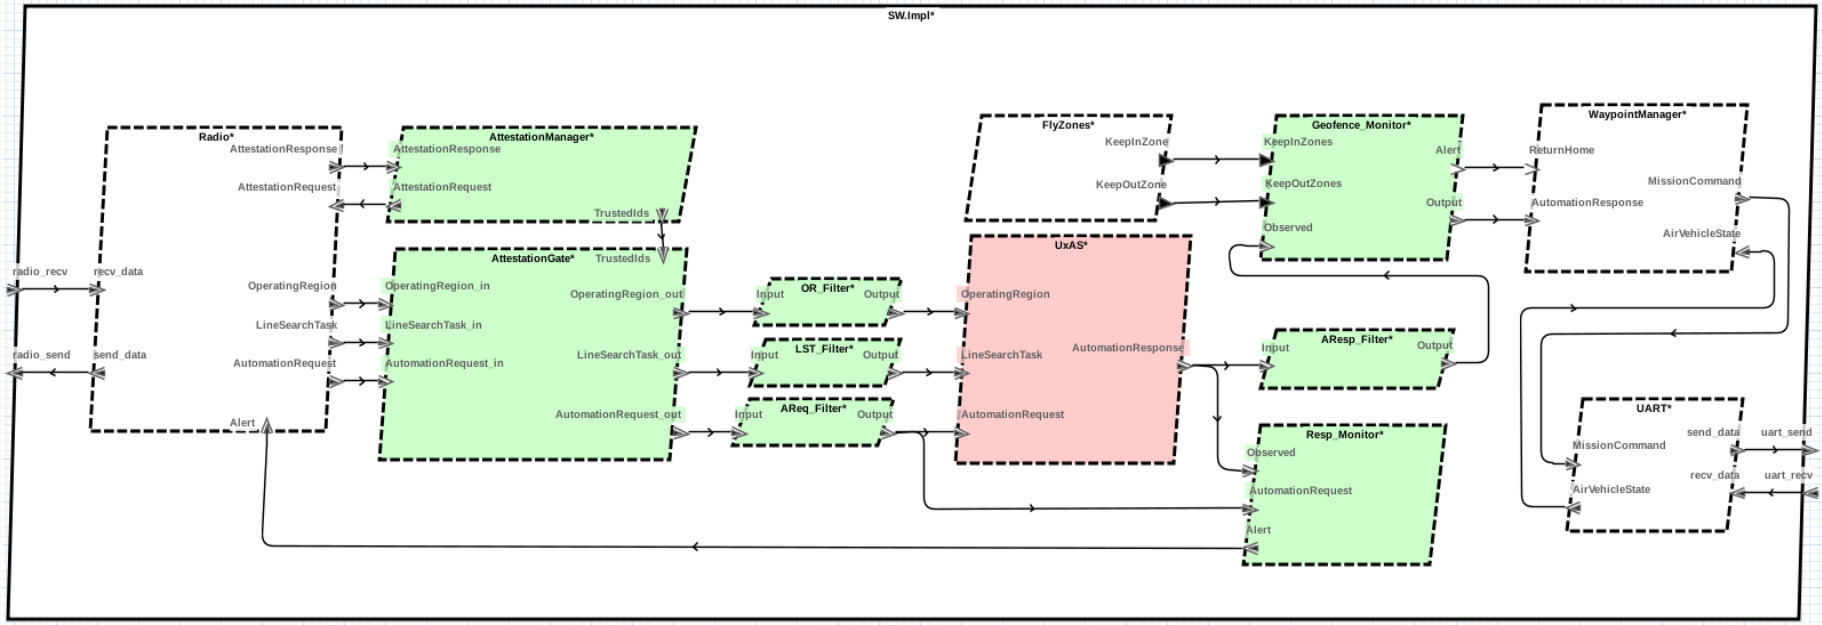
\includegraphics[width=1\columnwidth]{figs/hardened-sw.png}
	\caption{Cyber-resilient software architecture.} 
	\label{fig:hardened-sw} 
\end{figure}

Once we have determined that the model is correct and satisfies its cyber requirements, and the software components in the model have been implemented, either by SPLAT or other means, the system can be built and deployed.  We run the HAMR tool to generate the component stubs and infrastructure code necessary to enable component communication and execution according to a specified schedule.
HAMR translates the AADL system model to code that implements threading infrastructure and inter-component communication and is consistent with the AADL specification computational model.
%
HAMR then compiles the software to execute on seL4~\cite{sel4-2009}, a verified capability-based microkernel (accompanied by formal proof of spatial isolation properties down to the binary level).

The UAV and Ground Station software were deployed on the ODROID XU4 hardware and communicated with each other over Ethernet.  The AMASE flight simulator, representing the Flight Contol Computer was run on a Linux machine and connected to the UAV ODROID via a serial connection.  The UxAS implementation on the UAV was modified by adding malicious code that would prevent it from responding to Automation Requests or produce flight plans that would violate the operating region constraints.  Some of the Line Search Task messages transmitted from the Ground Station contained malformed messages that would modify the UxAS behavior. In addition, we modified the Ground Station to simulate a breach for the attestation test.

We performed an initial set of tests on the un-hardened system (Figure~\ref{fig:sw-initial}) to verify the effectiveness of the malicious code.  The following scenarios were exercised:

\paragraph{Infected Ground Station} In this scenario, one of the UxAS files is modified on the Ground Station. When Ground Station files are modified in such an unauthorized manner, messages sent to the UAV will be rejected by the Attestation Manager.  

\paragraph{Malformed Line Search Task message} In this scenario, the Line Search Task message contains a waypoint with a longitude value outside the permitted range.  Such malformed messages could exploit vulnerabilities in the onboard software.  This vulnerability is mitigated by inserting a well-formedness filter.  The filter prevents the Line Search Task message from reaching UxAS.

\paragraph{UxAS vulnerability exploit} In this scenario, Line Search Tasks with greater than 90 waypoints will trigger a vulnerability that will crash UxAS.   When this occurs, UxAS be prevented from generating an Automation Response.  This vulnerability is mitigated by inserting a Response Monitor, which checks to see that UxAS outputs an Automation Response message shortly after receiving an Automation Request.  For this scenario, we chose for the monitor to output a status message, which would then be received by the Ground Station and an appropriate action taken.

\paragraph{UxAS trojan modifies flight plan} In this scenario, a trojan embedded in UxAS will attempt to cause the UAV to fly into the specified keep-out zone by modifying the mission command waypoints in the Automation Response.  However, the UAV will detect that it is being instructed to fly into a keep-out zone and instead return to Home Base.

We repeated the tests on the hardened system and were able to demonstrate that our mitigations were successful, as indicated by the status messages sent from the high-assurance components, shown in Figure~\ref{fig:mitigation-output}.

\begin{figure}[h]
	\centering
	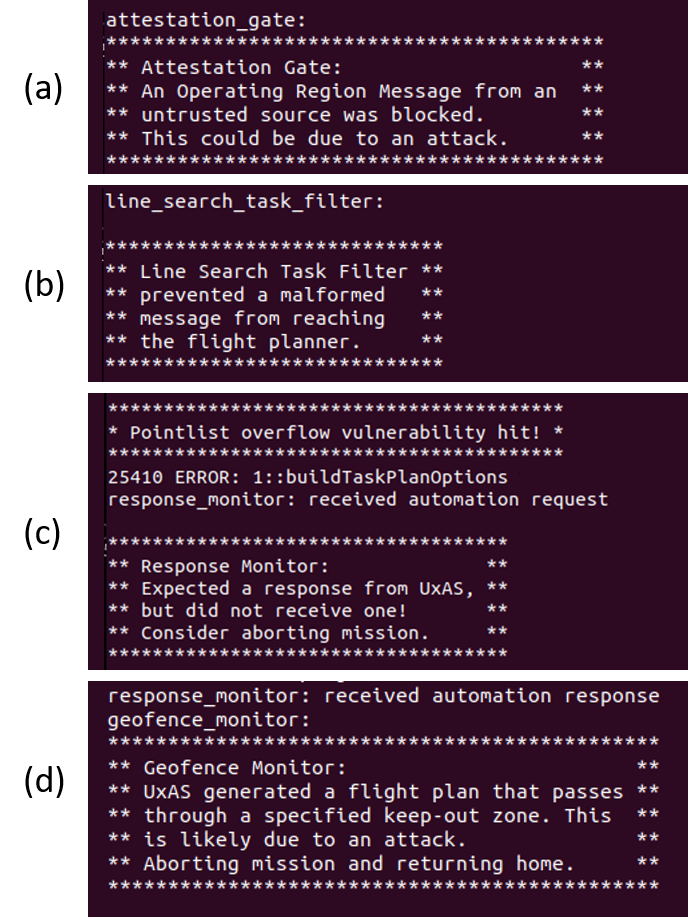
\includegraphics[width=0.8\columnwidth]{figs/mitigation-output.png}
	\caption{Cyber-resilient system response.} 
	\label{fig:mitigation-output} 
\end{figure}



\section{Related Work} \label{sec:related-work}
Assume-guarantee reasoning for compositional verification in reactive systems is well-studied \cite{10.1007/978-3-642-28891-3_13, composition1, 10.1145/2658982.2527272, 10.1007/978-3-319-17524-9_7}. Automated proofs of realizability for assume-guarantee reasoning are useful for engineers implementing components in the system \cite{10.1007/978-3-319-17524-9_13, 10.1007/978-3-319-29613-5_7}. Algorithms for actual component synthesis for Lustre models using k-induction or IC3/PDR provide an automated path from the assume-guarantee reasoning to an actual satisfying node implementation \cite{katis2017synthesis, 10.1007/978-3-319-89963-3_10}. These synthesis algorithms generate code in the Lustre modeling language but do not provide a path to a low-level implementation that could be fielded.

Contracts are similar to assume-guarantee reasoning but are targeted to programming languages. Contracts are often more expressive than assume-guarantee reasoning and can not only be stateful but higher-order \cite{10.1145/583852.581484}. As contracts are often written in the target language, synthesis is not a problem for monitoring but comes with significant overhead \cite{10.1007/978-3-642-28869-2_11}. A monitor for a contract can be removed when it can be statically proved that the code preserves the contract under all possible inputs and executions \cite{10.1145/3158139}.

\section{Conclusion} \label{sec:conclusion}
Cyber-physical systems must be tolerant to cyber-attacks in the same way they are tolerant to faults. The DARPA CASE program is creating an MBSE environment for designers to integrate cyber-vulnerability analysis and mitigation through the design process to harden systems early in the design process. BriefCASE is the result of that program, and it provides cyber-analysis tools that add cyber requirements to the AGREE specification for the design and architectural transforms with AGREE specifications to satisfy the cyber requirements. BriefCASE is fully integrated into the OSATE AADL modeling environment for ease of use by system engineers.

The filter architectural transformation in BriefCASE prevents malformed data from being propagated downstream to other components while the monitor transformation enforces temporal properties to detect when untrusted components behave maliciously. The components are specified by corresponding auto-generated AGREE contracts that only require the system designer to state the policies to enforce.These can be adapted from the cyber requirements in the system design. The specifications are automatically synthesized to CakeML that can then be compiled to a wide array of backend targets. The synthesis to CakeML is done in a way that preserves the meaning of the specifications.

The BriefCASE tool suite demonstrated in action on a full-scale case study with the UxAS open source UAV AI planning system. The complex system requires several architectural transformations to meet cyber-requirements, and the entire system is synthesized and deployed on the seL4 platform running on ODRIOD using the synthesis tool described here and the BriefCASE HAMR tool to generate the communication fabric. The size and scale of the case study gives some evidence that BriefCASE, with its transformations, scales to the complexity demands often seen in real-world design.

Ongoing work is using BriefCASE on the Collin' Common Avionics Architecture System (CAAS) in the context of a CH47 rotary wing platform \cite{caas}. The filter and monitor transformations are being employed to protect against \emph{Automatic Dependent Surveillance-Broadcast} (ADS-B) spoofing by malicious actors in the airspace. That work is expanding synthesis with uninterpreted functions to support non-linear and transcendental functions. Other ongoing work is mechanizing the synthesis proof in HOL4 and lifting the proof results given for finite streams to infinite streams.

\clearpage
\bibliographystyle{plain}
\bibliography{paper}

% \appendix
% \section{Contiguity Types}
% The formal specification of a component, and the synthesis of that specification, relies on \emph{contiguity types} to define the input and output data (cite contiguity). A contiguity type is a self-describing specification for messages. Its formalism has basis in formal languages. Similar to how a regular expression implies a set of words that form its language, so does a contiguity type specification imply a set of messages for its language where a message is a finite sequence of contiguous bytes (e.g., a string). 

What makes contiguity type specification more expressive than regular expressions is that it is self-describing meaning that the contents of the message itself may determine the rest of the message. An example is the \texttt{AutomationResponse} from the system in the previous section with its contiguity type specification.
{\small
\begin{verbatim}
  {TaskID : i64
   Length : u8
   Waypoints : Waypoint[Length]
  }
\end{verbatim}
}
\noindent The \texttt{Waypoints} array size depends on the value of \texttt{Length} so the actual number of bytes in the message depends on the contents of the message itself. 

The type specifications may also carry meta-information about the contents of the message.
{\small
\begin{verbatim}
  {Latitude : float
   lt-rng : Assert (-90 <= Latitude <= 90) 
   Longitude : float
   lng-rng : Assert (-180 <= Longitute <= 180)
   Altitude : float
   a-rng : Assert (10000 <= Altitude <= 15000)
  }
\end{verbatim}
}
\noindent Here the specification encodes the allowed ranges for each field of the waypoint. These assumptions restrict the resulting language to include only conforming messages and can be checked while constructing a message from a sequence of bytes. The notation $\LangTheta{\tau}$ denotes the language defined by the specification $\tau$ using the environment $\theta$ for expression evaluation.

Every contiguity type specification has a corresponding CakeML \emph{matcher} that when given a message string returns true or false if that message belongs to the language of the specification. If the message does belong to the language, an \emph{environment} is provided to access each part of the message. An environment, $\theta: \lval \mapsto \konst{string}$ binds \emph{L-values} to strings, where an L-value is an expression that can appear on the left hand side of an assignment (e.g., \texttt{AutomationRequest.Waypoints[0].Latitude}). 

The main result of contiguity types is the proof of the relationship between the language of the specification and the synthesized matcher from the specification that is summarized below.
\[
  \konst{match}\; s_1s_2 = \konst{SOME}(\theta, s_2)
  \imp \theta(\tau) \cdot s_2 = s_1s_2 \wedge s_1 \in \LangTheta{\tau}
\]
If there is a match on the substring $s_1$, then reconstituting the string from the resulting environment and concatenating it with $s_2$ yields the original string, and the matched string $s_1$ is in the language of the type specification.  

% \section{System Model and Semantics}
% A \emph{system} is a collection of \emph{components}, \emph{connections} between components, a \emph{scheduler} to order execution, and a \emph{system environment} for primary inputs. The computation for the component in this work is defined entirely by a step function:
\[
\konst{stepFn} : \mathit{inports} \times \mathit{stateVars} \to \mathit{stateVars}
\]
The scheduler \emph{activates} components in some order. Activating a component is defined as follows: 
\[
\begin{array}{ll}
 \mathit{inportVals} & = \konst{readInputs}(); \\
 (v_1,\ldots,v_k) & = \konst{readState}() ; \\
 ({v_1}',\ldots,{v_k}') & = \konst{stepFn} (\mathit{inportVals},\mathit{stateVars}) ; \\
 \multicolumn{2}{l}{\konst{writeState}({v_1}',\ldots,{v_k}');} \\
 \multicolumn{2}{l}{\konst{writeOutputs}({v_1}',\ldots,{v_k}');} \\
\end{array}
\]
It is assumed that the scheduler follows some sensible partial order of component activation and allows each component sufficient time for its computation.


\end{document}


